\documentclass[aspectratio=169]{beamer}
\usetheme{Bruno}
\usepackage{amsmath}
\usepackage{amssymb}
\usepackage{siunitx}
\usepackage{float}
\usepackage{tikz}
\def\checkmark{\tikz\fill[scale=0.4](0,.35) -- (.25,0) -- (1,.7) -- (.25,.15) -- cycle;} 
\usepackage{url}
\usepackage[siunitx,american,RPvoltages]{circuitikz}
\ctikzset{capacitors/scale=0.7}
\ctikzset{diodes/scale=0.7}
\usepackage{tabularx}
\newcolumntype{C}{>{\centering\arraybackslash}X}
\renewcommand\tabularxcolumn[1]{m{#1}}% for vertical centering text in X column
\usepackage{tabu}
\usepackage[spanish,es-tabla,activeacute]{babel}
\usepackage{babelbib}
\usepackage{booktabs}
\usepackage{pgfplots}
\usepackage{hyperref}
\hypersetup{colorlinks = true,
            linkcolor = black,
            urlcolor  = blue,
            citecolor = blue,
            anchorcolor = blue}
\usepgfplotslibrary{units, fillbetween} 
\pgfplotsset{compat=1.16}
\usepackage{bm}
\usetikzlibrary{arrows, arrows.meta, shapes, 3d, perspective, positioning,mindmap,trees,backgrounds}
\renewcommand{\sin}{\sen} %change from sin to sen
\usepackage{bohr}
\setbohr{distribution-method = quantum,insert-missing = true}
\usepackage{elements}
\usepackage{verbatim}
\usepackage[edges]{forest}
\usepackage{etoolbox}
\usepackage{schemata}
\usepackage{appendix}
\usepackage{listings}

\definecolor{color_mate}{RGB}{255,255,128}
\definecolor{color_plas}{RGB}{255,128,255}
\definecolor{color_text}{RGB}{128,255,255}
\definecolor{color_petr}{RGB}{255,192,192}
\definecolor{color_made}{RGB}{192,255,192}
\definecolor{color_meta}{RGB}{192,192,255}
\newcommand\diagram[2]{\schema{\schemabox{#1}}{\schemabox{#2}}}

\definecolor{codegreen}{rgb}{0,0.6,0}
\definecolor{codegray}{rgb}{0.5,0.5,0.5}
\definecolor{codepurple}{rgb}{0.58,0,0.82}
\definecolor{backcolour}{rgb}{0.95,0.95,0.92}

\lstdefinestyle{mystyle}{
    backgroundcolor=\color{backcolour},   
    commentstyle=\color{codegreen},
    keywordstyle=\color{magenta},
    numberstyle=\tiny\color{codegray},
    stringstyle=\color{codepurple},
    basicstyle=\ttfamily\footnotesize,
    breakatwhitespace=false,         
    breaklines=true,                 
    captionpos=b,                    
    keepspaces=true,                 
    numbers=left,                    
    numbersep=5pt,                  
    showspaces=false,                
    showstringspaces=false,
    showtabs=false,                  
    tabsize=2
}

\lstset{style=mystyle}
\title{Instrumentación I: \\ \emph{Medidas de Propiedades}\\ \emph{Ópticas}}
\author{
    Juan J. Rojas, Hugo Sanchez Ortiz
}
\institute{Instituto Tecnológico de Costa Rica}
\date{\today}
\background{fig/background.jpg}
\begin{document}
\sisetup{unit-math-rm=\mathrm,math-rm=\mathrm} % change sinitx font
\sisetup{output-decimal-marker = {,}}
\maketitle

\newcommand{\blackandwhite}{white} %change this at the end

\begin{frame}{Luz}
        \begin{columns}[c, onlytextwidth]
        \begin{column}{0.55\textwidth}
            \begin{itemize}
                \item La luz es la parte de la radiación electromagnética que puede ser vista por el ojo humano. 
                \item  La luz, como todas las radiaciones electromagnéticas, está formada por partículas elementales desprovistas de masa denominadas fotones, cuyas propiedades de acuerdo con la dualidad onda-partícula explican las características de su comportamiento físico.
                \item Puede detectar una gran variedad de estímulos. 
            \end{itemize}
        \end{column}
        \begin{column}{0.45\textwidth}
            \centering
            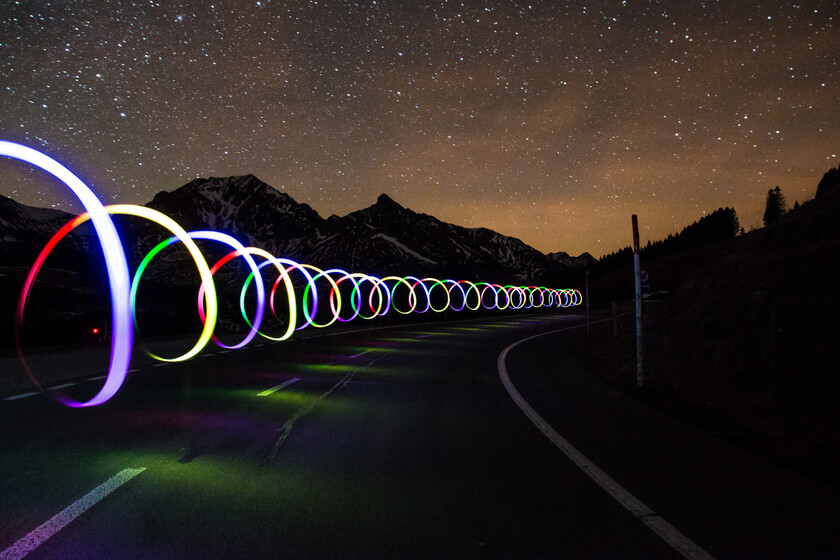
\includegraphics[width = 0.9\linewidth]{fig/Optica/Luz.jpg}
            
            \tiny{Tomado de \href{https://www.xataka.com/espacio/que-viajar-a-velocidad-luz-teoricamente-imposible-1}{Xataka}}
            
        \end{column}
    \end{columns}
\end{frame}


\begin{frame}{Luz}
\begin{columns}[c, onlytextwidth]
        \begin{column}{0.55\textwidth}
            \begin{itemize}
                \item Los fenómenos de reflexión, refracción, absorpción, interferencia, polarización y velocidad son herramientas poderosas de medición. 
                \item  Cuando la luz se forma, puede ser manipulada en múltiples formas. Como cambios de dirección, filtros de longitud de onda.
                \item El reto para el diseñador consiste en relacionar los estímulos de recibidos por la señal de luz en señales eléctricas.
            \end{itemize}
        \end{column}
        \begin{column}{0.45\textwidth}
            \centering
            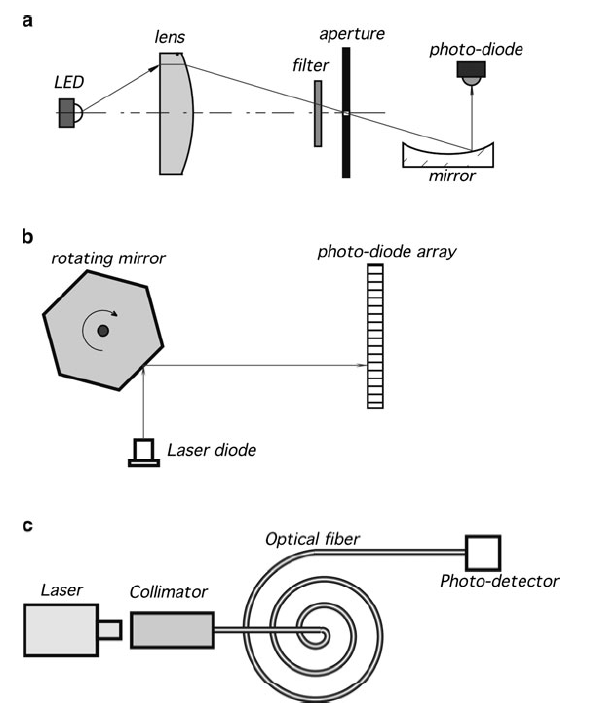
\includegraphics[width = 0.8\linewidth]{fig/Optica/UsosRefracccion_Radiacion.PNG}
            
            \tiny{Tomado de \cite{Fraden_2016}}
            \tiny{Ejemplos de sistemas ópticos que usan refracción (a) y reflexión (a,b,c)}
            
        \end{column}
    \end{columns}
\end{frame}

\begin{frame}{Luz, ¿onda o partícula?}
\begin{columns}[c, onlytextwidth]
        \begin{column}{0.45\textwidth}
            \centering
            \includegraphics[width = 1\linewidth]{fig/Optica/onda-partícula.png}\\
             \tiny{Tomado de: \href{https://www.bbc.com/mundo/noticias-52815076}{Física cuántica: qué es la dualidad partícula-onda de la luz y cómo su descubrimiento revolucionó la ciencia}}
        \end{column}
        \begin{column}{0.55\textwidth}
            \begin{itemize}
                \item Una partícula elemental presentan una dualidad onda-partícula. 
                \item  La propagación del espectro electromagnético, pero las composición sólo se da en paquetes de energía llamado fotones.
                \item El fotón tiene una masa de cero y una velocidad $c$ y cuando interactúa con materia, trabaja con energía: \\
                \centering
                $E=\frac{hc}{\lambda}$
            \end{itemize}
        \end{column}
    \end{columns}
\end{frame}

\begin{frame}{Espectro Electromagnético y Óptico}
\begin{columns}[c, onlytextwidth]
        \begin{column}{0.4\textwidth}
            \centering
            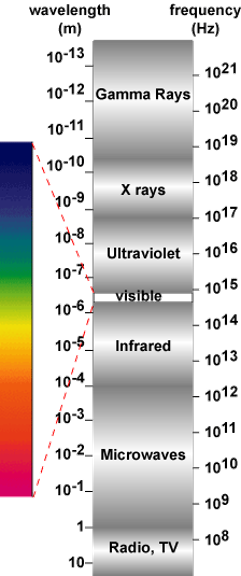
\includegraphics[width = 0.48\linewidth]{fig/Optica/Espectro.png}\\
        \end{column}
        \begin{column}{0.6\textwidth}
            \begin{itemize}
                \item La luz que vemos todos los días, es sólo una fracción de la luz de la energía total emitida por el Sol. 
                \item  Max Planck propuso que la energía total de la luz está compuesta por elementos indistingibles de energía.
                \item Albert Einstein realizó estudios sobre el efecto fotoeléctrico, logró distinguir esos paquetes de elementos cuánticos de energía.
            \end{itemize}
        \end{column}
    \end{columns}
\end{frame}

\begin{frame}{Espectro Electromagnético y Óptico}
            \centering
            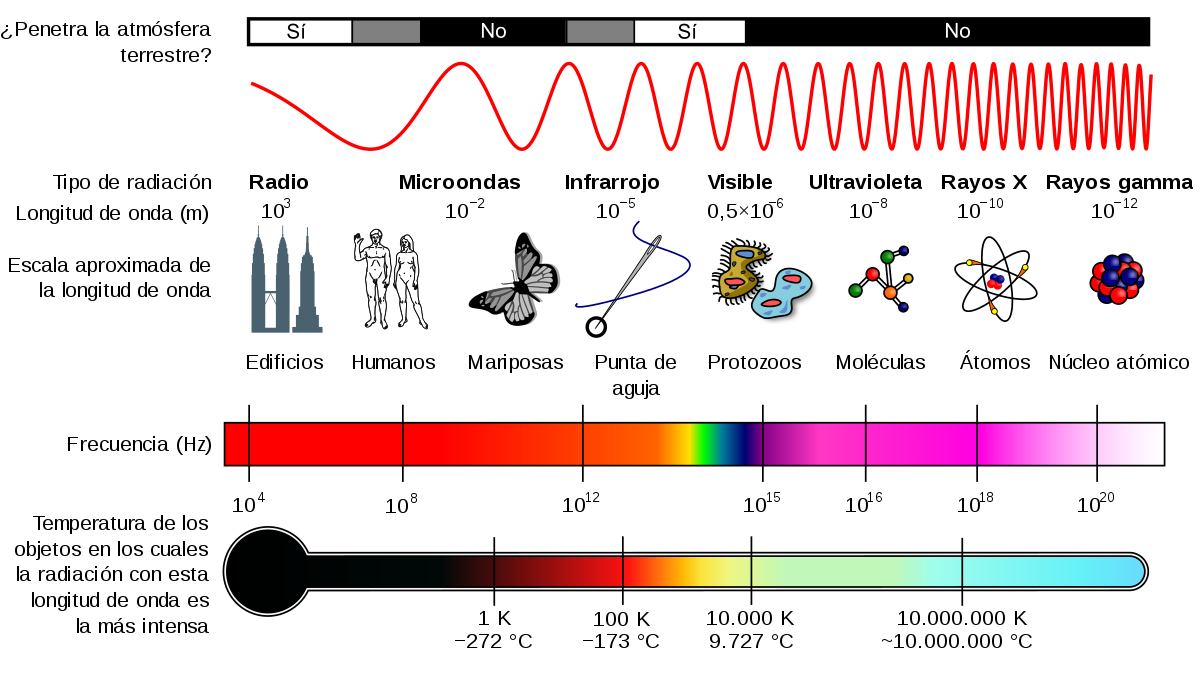
\includegraphics[width = 0.8\linewidth]{fig/Optica/1200px-EM_Spectrum_Properties_es.svg.png}\\
            \tiny{Tomado de: \href{https://es.wikipedia.org/wiki/Espectro_visible}{Wikicommons}}
\end{frame}

\begin{frame}{Espectro Óptico}
            \begin{itemize}
                \item El espectro óptico es una pequeña parte del total del espectro electromagnético.
            \end{itemize}
            \centering
            
            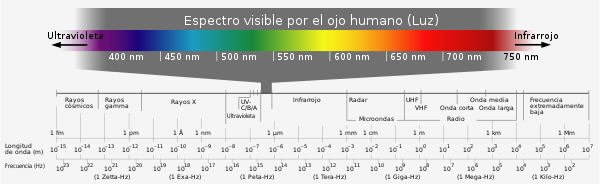
\includegraphics[width = 1\linewidth]{fig/Optica/Espectro Visible.png}\\
            \tiny{Tomado de: \href{https://es.wikipedia.org/wiki/Espectro_electromagnético}{Wikicommons}}
\end{frame}


\begin{frame}{Conceptos Básicos de las ondas}
    \begin{columns}[c, onlytextwidth]
        \begin{column}{0.55\textwidth}
            \begin{itemize}
                \item La luz como onda electromagnética, se caracteriza por una combinación de variación temporal de \textbf{E} (campo eléctrico) y \textbf{H} (campo magnético) propagándose por el espacio.
                \item La luz tiene una velocidad definida  por $c= 299 792 458 \frac{m}{s}$
                \item Si la luz se propaga en otro medio, se tiene que la velocidad está dada por:
                \begin{equation*}
                    v=\frac{c}{n}
                \end{equation*}
                Donde: $n=\sqrt{\epsilon_r \mu_r}$
            \end{itemize}
        \end{column}
        \begin{column}{0.45\textwidth}
            \centering
            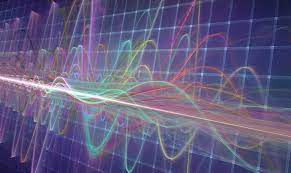
\includegraphics[width = 0.8\linewidth]{fig/Optica/ondas.jpg}\\
            \tiny{Tomado de: \href{https://www.viasat.com/es-mx/acerca-de-nosotros/sala-de-prensa/blog/que-son-las-ondas-de-radio-y-como-las-usan-los-satelites/}{Acá}}
        \end{column}
    \end{columns}
\end{frame}

\begin{frame}{Conceptos Básicos de las ondas}
    \begin{columns}[c, onlytextwidth]
        \begin{column}{0.55\textwidth}
            \begin{itemize}
            \item Propiedades de la luz como onda
            \begin{enumerate}
                \item Amplitud (A)
                \item Longitud de onda ($\lambda$)
                \item Frecuencia (f) 
                \begin{equation*}
                    f=\frac{1}{T}
                \end{equation*}
                \item Velocidad (V)
                \begin{equation*}
                    V=\frac{\lambda}{f}
                \end{equation*}
                
                \begin{equation*}
                    \lambda=\frac{c}{f}
                \end{equation*}
            \end{enumerate}
            
            \end{itemize}
        \end{column}
        \begin{column}{0.45\textwidth}
            \centering
            \centering
            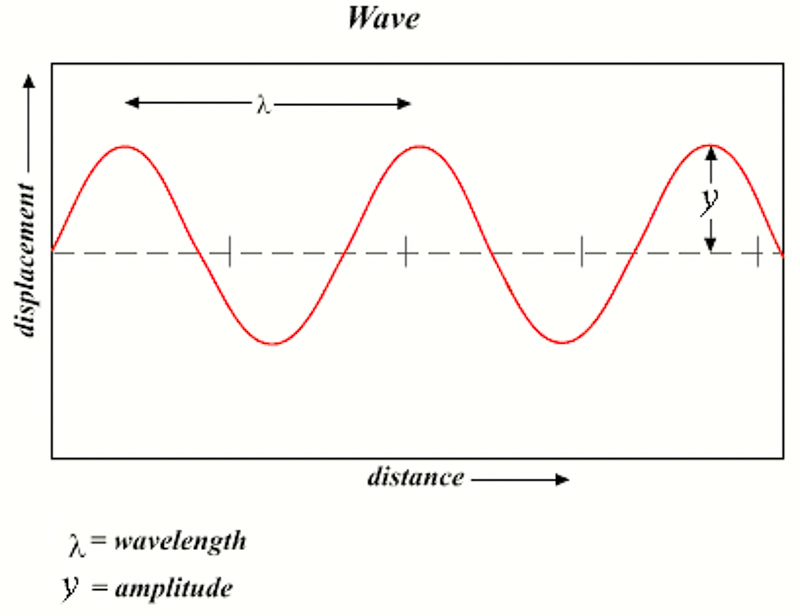
\includegraphics[width = 1\linewidth]{fig/Optica/amplitud.jpg}
            \vspace{0.5cm}
            
            \tiny{Tomado de \cite{Fraden_2016}}
            
            \tiny{Amplitud y longitud de onda}
        \end{column}
    \end{columns}
\end{frame}

\begin{frame}{Conceptos Básicos de las ondas}
\begin{itemize}
    \item La longitud de onda tiene una relación inversa con la frecuencia, a mayor frecuencia, menor longitud de onda, y viceversa.
\end{itemize}
 \begin{table}[]
 \footnotesize
    \centering
    \begin{tabular}{m{3.2cm} m{0.8cm} m{0.8cm} m{0.8cm} m{0.8cm} m{0.8cm} m{0.8cm} m{0.8cm} m{0.8cm} }
        \toprule
        \textbf{Longitud de onda (nm)} & 10 & 300 & 390 & 492 & 622 & 770 & 6000 & 100000\\
        \midrule
        \textbf{Frecuencia(THz)} & 30000 & 999 & 769 & 609 & 482 & 389 & 50 & 3  \\

        \bottomrule
    \end{tabular}
    \tiny{\caption{Espectro luminoso $\lambda (nm)$ vs $frec (THz)$} \cite{sole2005instrumentacion}}
    \label{Longitud vs Frecuencia}
    \normalsize
    \begin{itemize}
    \item Además existen fenómenos que pueden alterar dicha composición.
\end{itemize}
\end{table}
    
\end{frame}


\begin{frame}{Refracción, reflexión, atenuación y dispersión}
    \begin{columns}[c, onlytextwidth]
        \begin{column}{0.55\textwidth}
            \begin{itemize}
                \item La luz puede manipularse de distintas formas.
                \item La primera de las manipulaciones que puede realizarse es geométrica, es decir en función de la trayectoria. 
                \item Existen distintos métodos a estudiar: 
                \begin{itemize}
                    \item \textbf{Refracción}
                    \item \textbf{Reflexión}
                    \item \textbf{Atenuación}
                    \item \textbf{Dispersión}
                \end{itemize}
            \end{itemize}
        \end{column}
        \begin{column}{0.45\textwidth}
            \centering
            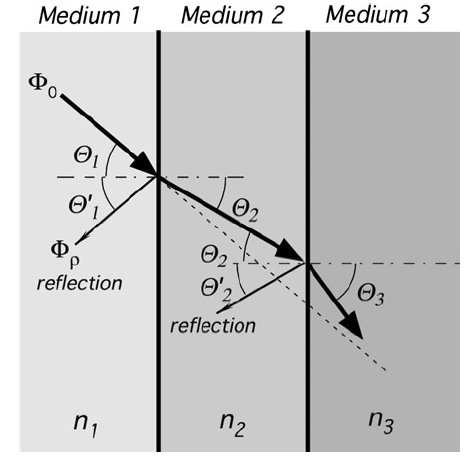
\includegraphics[width = 0.9\linewidth]{fig/Optica/Radiometry.PNG}
            
            \tiny{Tomado de \cite{Fraden_2016}}
            
            \tiny{Luz pasando por distintos materiales con distintos índices refractivos}
        \end{column}
    \end{columns}
\end{frame}

\begin{frame}{Refracción}
    \begin{columns}[c, onlytextwidth]
        \begin{column}{0.55\textwidth}
            \begin{itemize}
                \item La refracción es el cambio de dirección de la luz cuando pasa a un material de índice de refracción diferente $n$
                \item Está definido por:\\
                \begin{equation*}
                     n=\frac{Velocidad de la luz en el aire}{velocidad de luz en el medio}
                \end{equation*}
               
                \item Algunos materiales: 
                \begin{itemize}
                    \item  $n_{aire}=1$
                    \item  $n_{agua}=1.33$
                    \item $n_{vidrio}=1.65$
                \end{itemize}
            \end{itemize}
        \end{column}
        \begin{column}{0.45\textwidth}
            \centering
            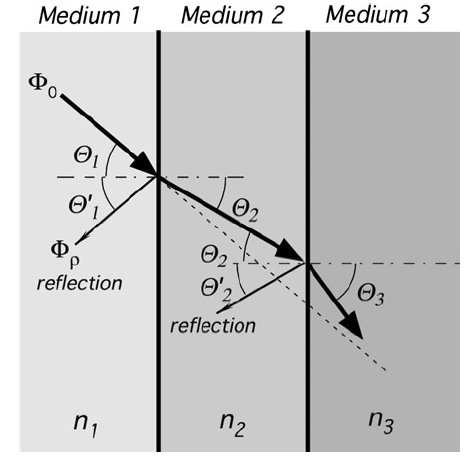
\includegraphics[width = 0.9\linewidth]{fig/Optica/Radiometry.PNG}
            
            \tiny{Tomado de \cite{Fraden_2016}}
            
            \tiny{Luz pasando por distintos materiales con distintos índices refractivos}
        \end{column}
    \end{columns}
\end{frame}

\begin{frame}{Refracción}
    \begin{columns}[c, onlytextwidth]
        \begin{column}{0.55\textwidth}
            \begin{itemize}
                \item Cuando un rayo de luz viaja de un medio a otro en Ángulo de salida  $\theta_2$ , depende de las propiedades de los medios y el Ángulo de entrada $\theta_1$. Además, de la velocidad del medio1 $v_1$ y velocidad del medio2 $v_2$.
                \item Está definido por:\\
                \begin{equation*}
                     \frac{sin \theta_2}{sin \theta_2}=\frac{v_2}{v_1}
                \end{equation*}
               
                \item cuando un rayo de luz se desplaza de un medio1 con velocidad v1 más alta que la del medio2 (v2), el ángulo $\theta_2$ es menor que ángulo de incidencia
            \end{itemize}
        \end{column}
        \begin{column}{0.45\textwidth}
            \centering
            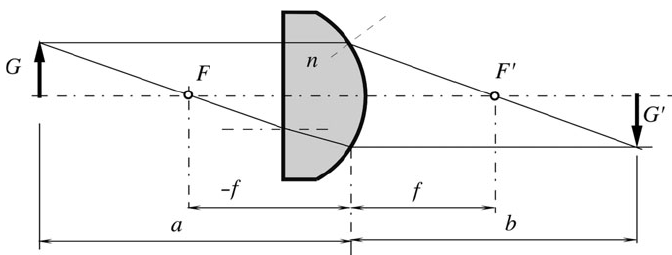
\includegraphics[width = 0.9\linewidth]{fig/Optica/lense.PNG}
            
            \tiny{Tomado de \cite{Fraden_2016}}
            
            \tiny{Geometría para un lente convexo}
        \end{column}
    \end{columns}
\end{frame}

\begin{frame}{Reflexión}
    \begin{columns}[c, onlytextwidth]
    \begin{column}{0.45\textwidth}
            \centering
            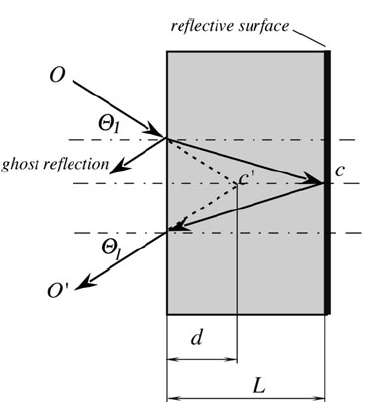
\includegraphics[width = 0.9\linewidth]{fig/Optica/reflection.PNG}
            \tiny{Tomado de \cite{Fraden_2016}}
            \tiny{Espejo en segunda interfaz}
        \end{column}
        \begin{column}{0.55\textwidth}
            \begin{itemize}
                \item La reflexión es el fenómeno más antiguo en ser utilizado.
                \item En todo proceso de transporte de luz existe un fenómeno de reflexión.
                \item Si la reflexión ocurre en una superficie lisa, se le denomina reflexión especular, si es una superficie rugosa, se le conoce como reflexión difusa. 
                \item Un caso interesante es la reflexión total interna (\textbf{TIR})
            \end{itemize}
        \end{column}
    \end{columns}
\end{frame}

\begin{frame}{Reflexión}
            \centering
            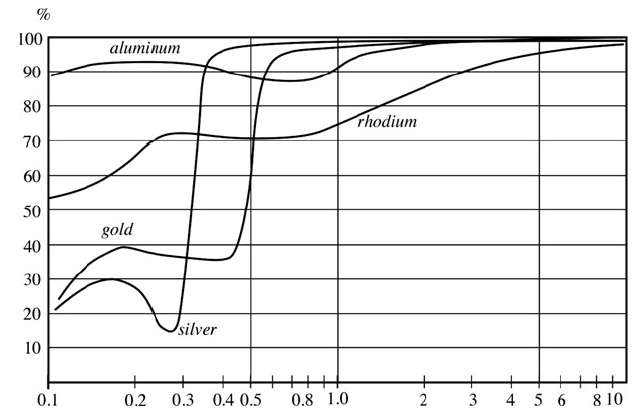
\includegraphics[width = 0.7\linewidth]{fig/Optica/Reflectance_materials.PNG}\\
            \tiny{Tomado de \cite{Fraden_2016}}
            \tiny{Reflectancia espectral de algunos materiales}

\end{frame}

\begin{frame}{Atenuación}
    \begin{columns}[c, onlytextwidth]
        \begin{column}{0.55\textwidth}
            \begin{itemize}
                \item La luz cuando se propaga, puede perder energía con la distancia.
                \item La atenuación se mide en \textit{decibelios dB}
                \begin{equation*}
                     atenuacion= 10 (log\frac{P_0}{P_i})
                \end{equation*}
                Donde $P_0$ es la potencia de salida y $P_i$ es la potencia de entrada. 
               
                \item Cuando un rayo de luz viaja entre dos puntos cualesquiera, su trayectoria es aquella que necesita el menor tiempo
            \end{itemize}
        \end{column}
        \begin{column}{0.45\textwidth}
            \centering
            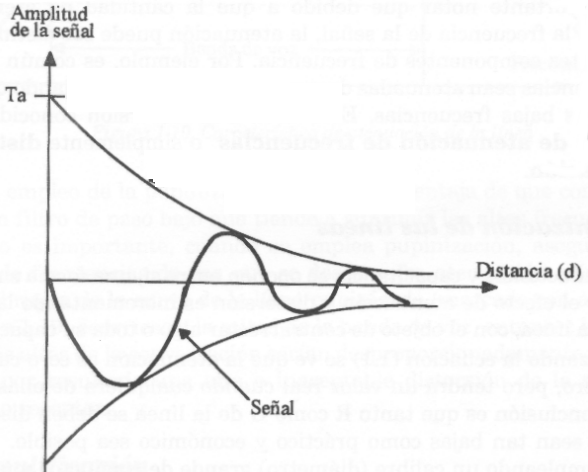
\includegraphics[width = 0.9\linewidth]{fig/Optica/atenuacion.png}
            
            \tiny{Tomado de \cite{Fraden_2016}}
            
            \tiny{Atenuación de una onda}
        \end{column}
    \end{columns}
\end{frame}

\begin{frame}{Dispersión}
    \begin{columns}[c, onlytextwidth]
    \begin{column}{0.45\textwidth}
            \centering
            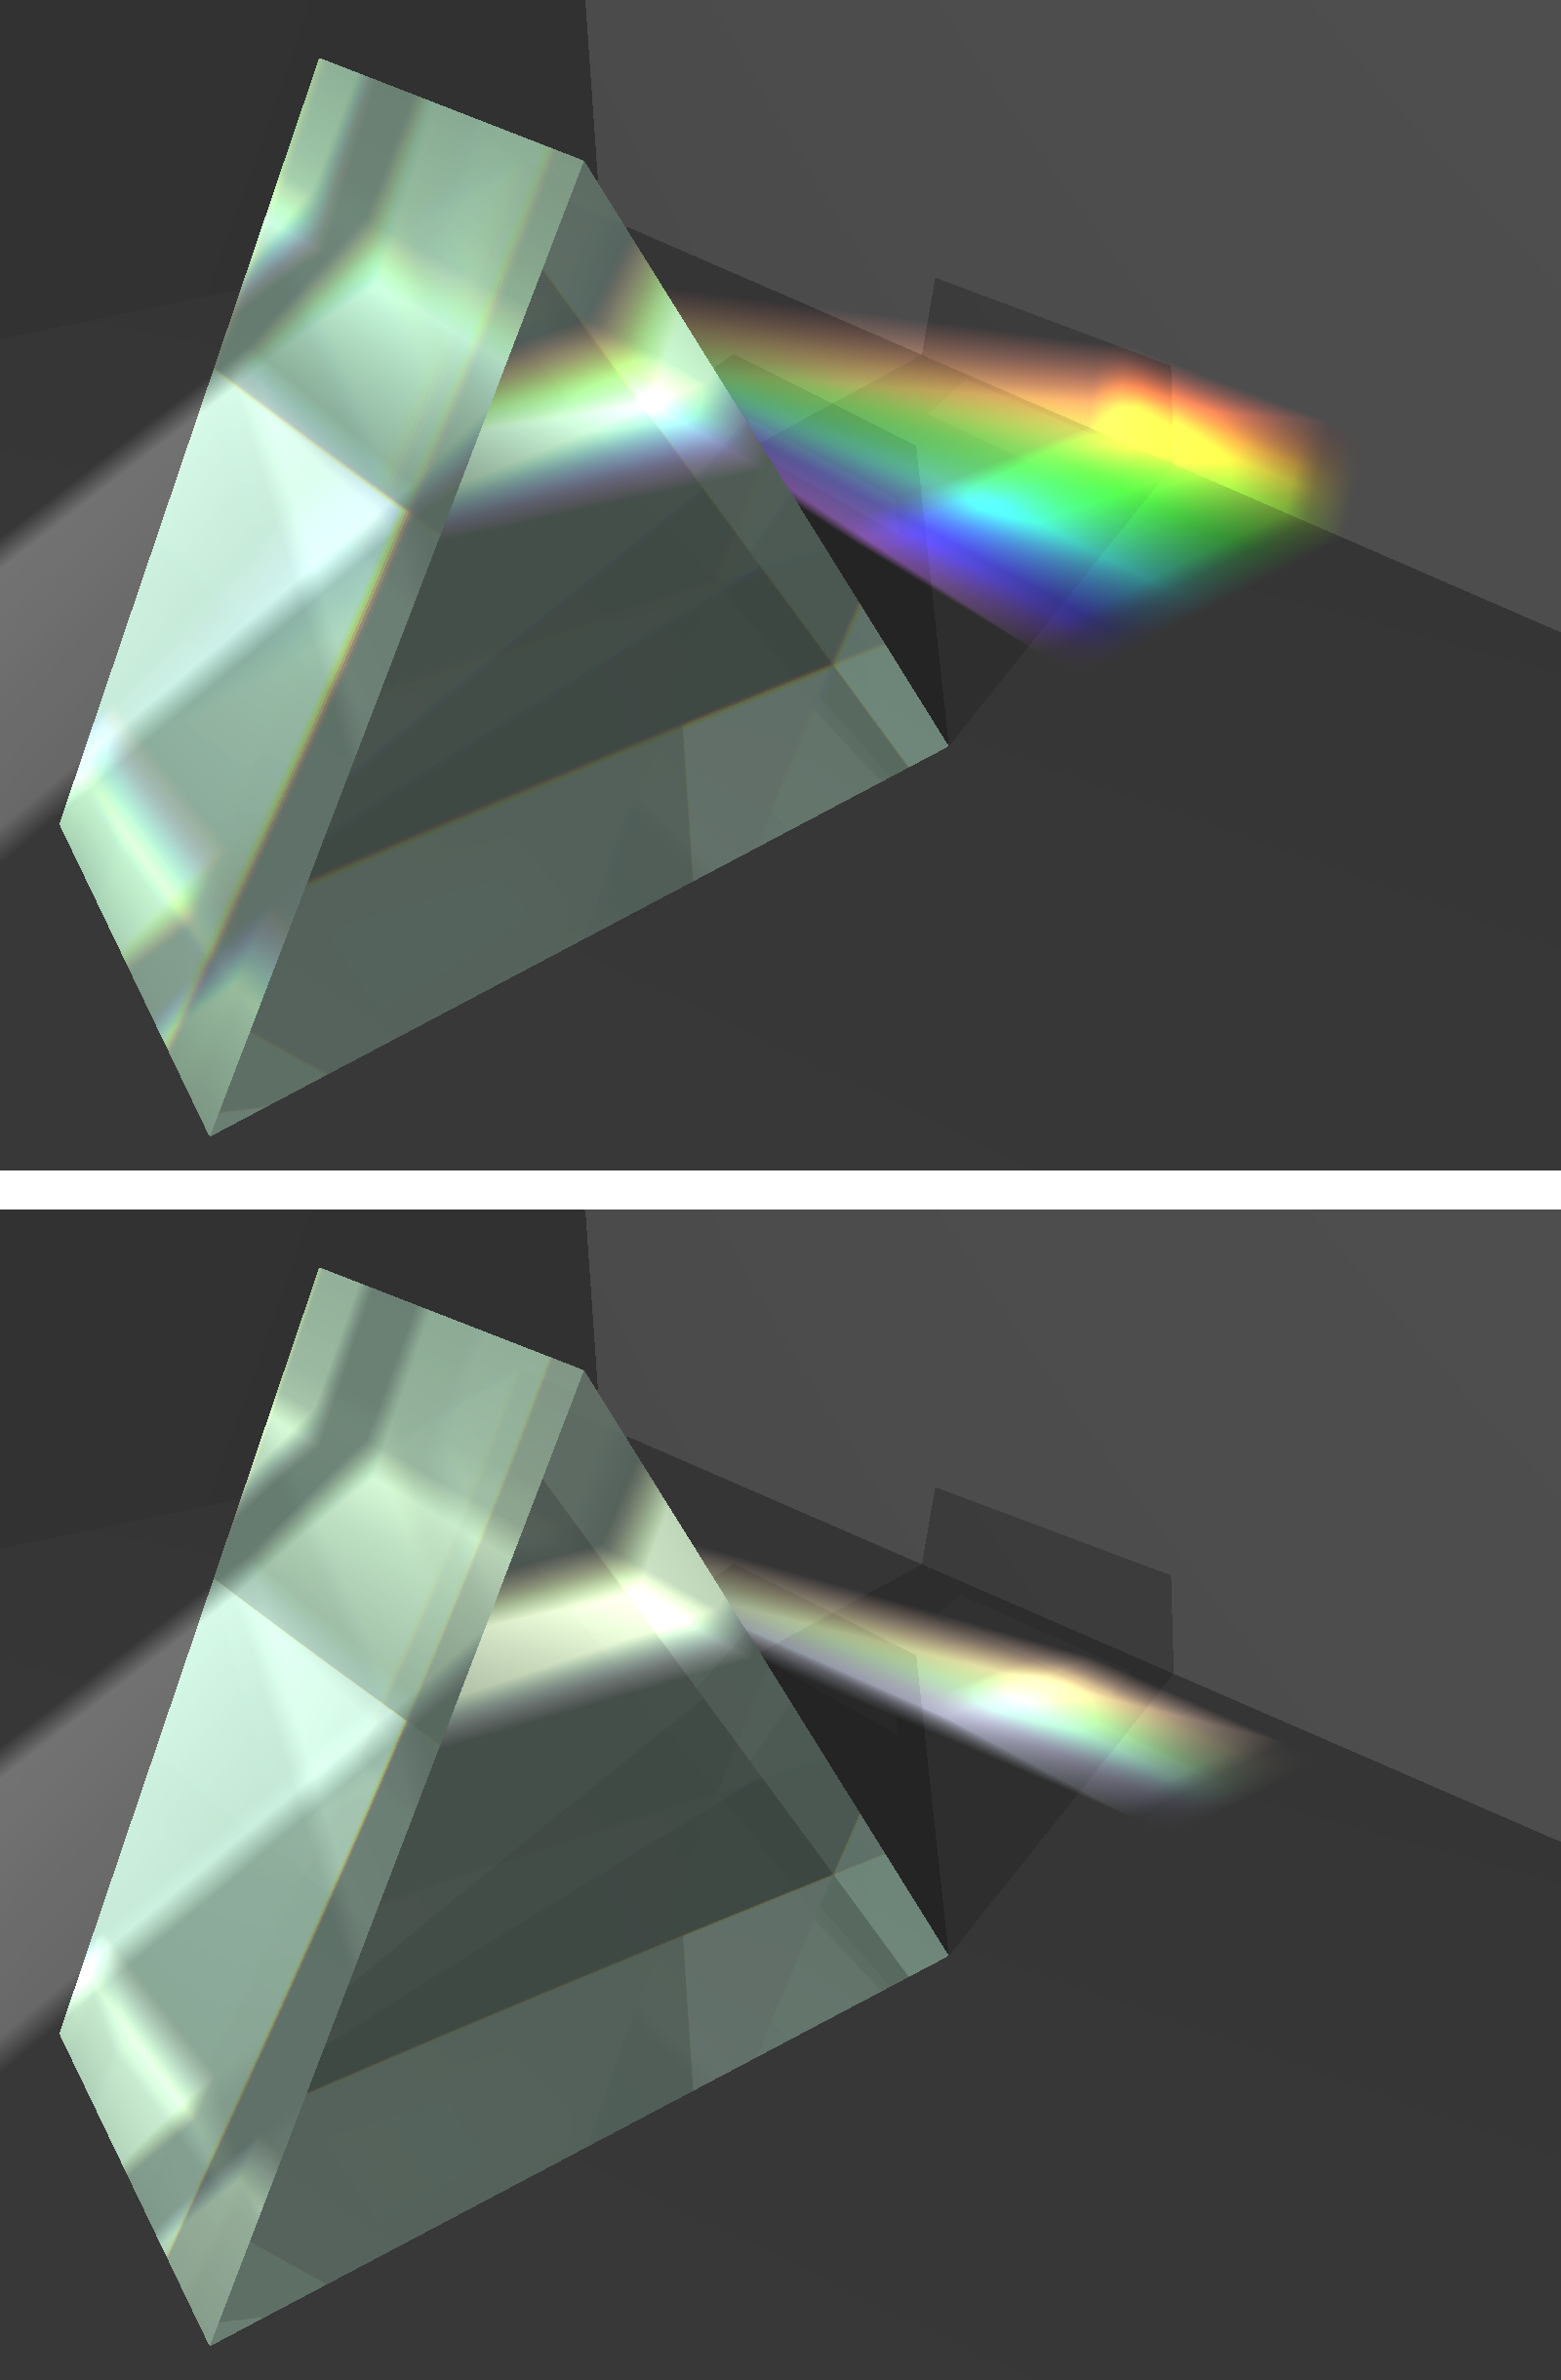
\includegraphics[width = 0.7\linewidth]{fig/Optica/Prisms_with_high_and_low_dispersion.png}\\
            \tiny{Tomado de: \href{https://es.wikipedia.org/wiki/Dispersición_refractiva}{Wikicommons}}
        \end{column}
        \begin{column}{0.55\textwidth}
            \begin{itemize}
                \item Todas las emisiones electromagnéticas tienen la capacidad de viajar a la misma velocidad en el vacío.
                \item Sin embargo, la velocidad cambia cuando deben atravesar otro material.
                \item Dicho fenómeno es dependiente de la longitud de onda, para el espectro visible.
                \begin{equation*}
                    1 < n_{\lambda_{rojo}} < n_{\lambda_{amarillo}} < n_{\lambda_{azul}}
                \end{equation*}
            \end{itemize}
        \end{column}
    \end{columns}
\end{frame}

\begin{frame}{Refracción, reflexión, atenuación y dispersión}
            \centering
            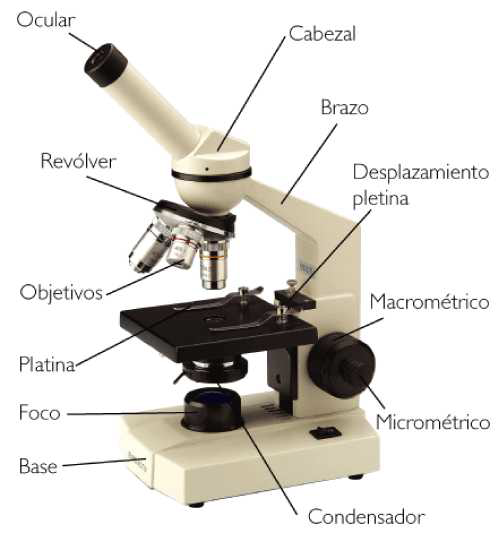
\includegraphics[width = 6cm]{fig/Optica/microscopio_optico.png}\\
            \tiny{Tomado de: \href{https://www.pardell.es/microscopia-optica.html}{Acá}}

\end{frame}


\begin{frame}{Absorción, fotoconductividad y efecto fotoeléctrico}
    \begin{columns}[c, onlytextwidth]
        \begin{column}{0.6\textwidth}
            \begin{itemize}
                \item Los mecanismos físicos tratan sobre la conversión de energía en materiales semiconductores.
                \item La combinación de las propiedades de un semiconductor, con las propiedades de transporte de luz, dan paso a aplicaciones sofisticadas a nivel de instrumentación.
            \end{itemize}
        \end{column}
        \begin{column}{0.40\textwidth}
            \centering
            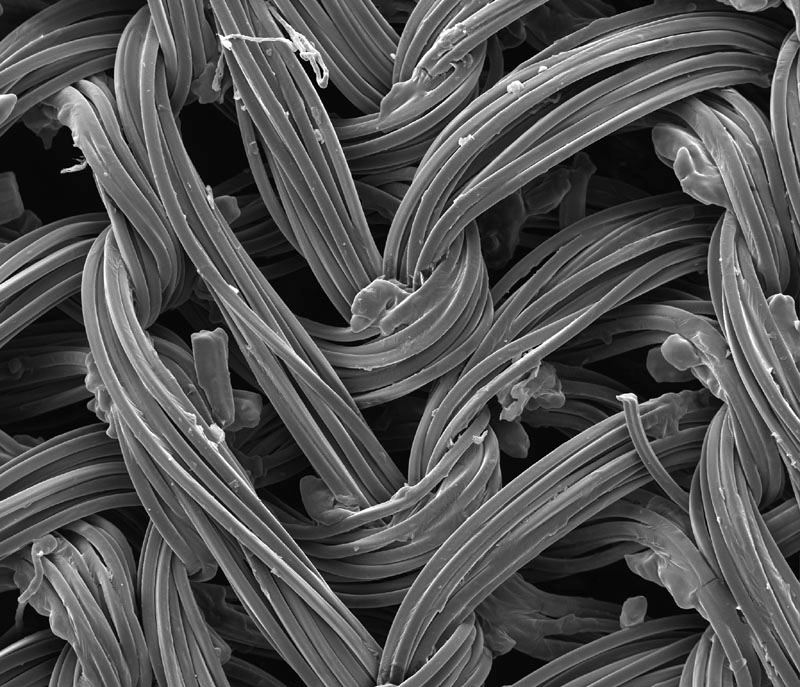
\includegraphics[width = 0.9\linewidth]{fig/Optica/barrido electronico.jpg}\\
            \tiny{Tomado de \href{https://todoenpolimeros.com/2019/01/07/microscopio-electronico-de-barrido/}{acá}}
        \end{column}
    \end{columns}
\end{frame}

\begin{frame}{Absorción, fotoconductividad y efecto fotoeléctrico}
    \centering
    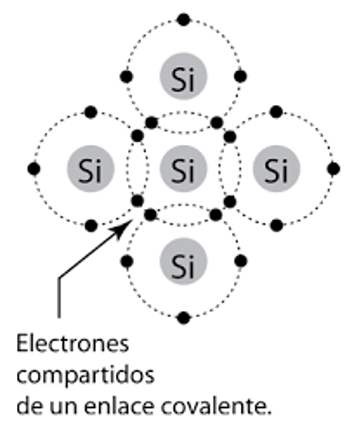
\includegraphics[width=5.5cm]{fig/Optica/Silicon.png}
\end{frame}

\begin{frame}{Absorción}
    \begin{columns}[c, onlytextwidth]
        \begin{column}{0.55\textwidth}
            \begin{itemize}
                \item La luz, al trabajar en paquetes de energía, tiene la capacidad de ser absorbida por el material.
                \item En muchos materiales esta absorción permite la generación de un par electrón hueco.
                \item Cada fotón genera una transición entre la banda de valencia (VB) hacia la banda de conducción (CB).
                \item La generación de un estímulo interno se realizará sí la energía es mayor a la de la banda prohibida:
                \begin{equation*}
                    E_G=E_C-E_v
                \end{equation*}

            \end{itemize}
        \end{column}
        \begin{column}{0.45\textwidth}
            \centering
    \includegraphics[width = 1\linewidth]{fig/Optica/Absorción.png}\\
            \tiny{Tomado de \cite{Fraden_2016}}
            \tiny{Fotoefecto en un semiconductor}
        \end{column}
    \end{columns}
\end{frame}

\begin{frame}{Fotoconductividad}
    \begin{columns}[c, onlytextwidth]
        \begin{column}{0.55\textwidth}
            \begin{itemize}
                \item Es un efecto optoelectrónico en el que un material se vuelve más conductor de electricidad debido a la absorción de la radiación electromagnética.
                \item La absorpción de la luz en los semiconductores pueden liberar portadores de carga que contribuyen al proceso de conducción, produciéndose la conversión de señales ópticas en eléctricas.
                \end{itemize}
        \end{column}
        \begin{column}{0.45\textwidth}
            \centering
    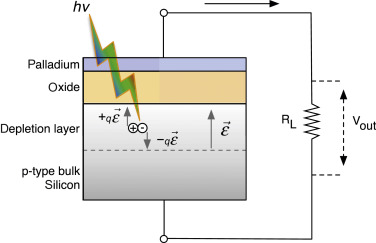
\includegraphics[width = 1\linewidth]{fig/Optica/photocondutivity.jpg}\\
            \tiny{Tomado de \href{https://www.sciencedirect.com/topics/materials-science/photoconductivity/}{Science Direct}}
        \end{column}
    \end{columns}
\end{frame}

\begin{frame}{Efecto fotoeléctrico}
    \begin{columns}[c, onlytextwidth]
        \begin{column}{0.55\textwidth}
            \begin{itemize}
                \item La emisión de electrones por un material al incidir sobre él una radiación electromagnética (luz visible o ultravioleta, en general).
                \item Los fotones del rayo de luz tienen una energía característica determinada por la frecuencia de la luz. En el proceso de fotoemisión, si un electrón absorbe la energía de un fotón y este último tiene más energía que la función de trabajo, el electrón es arrancado del material. Si la energía del fotón es demasiado baja, el electrón no puede escapar de la superficie del material.

            \end{itemize}
        \end{column}
        \begin{column}{0.45\textwidth}
            \centering
    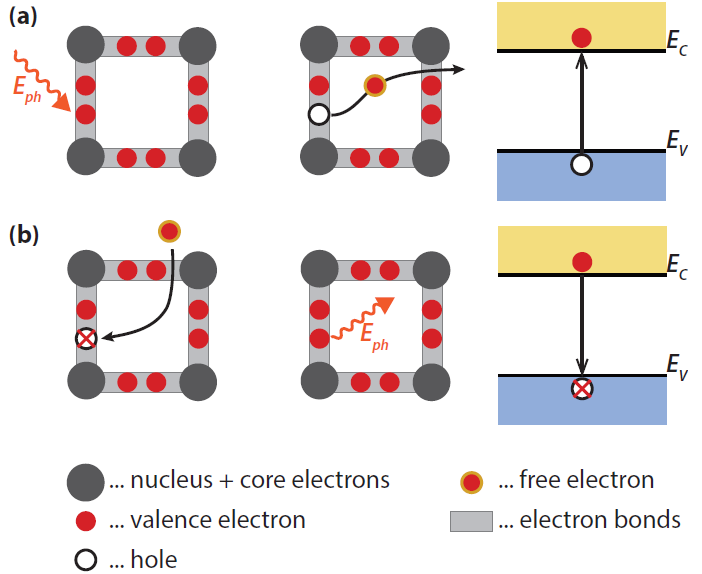
\includegraphics[width = 1\linewidth]{fig/Optica/Fotoefecto.png}\\
            \tiny{Tomado de \cite{Fraden_2016}}
            \tiny{Efecto Fotoeléctrico en un semiconductor}
        \end{column}
    \end{columns}
\end{frame}

\begin{frame}{Dispositivos opto electrónicos y sensores}
    \begin{columns}[onlytextwidth]
        \begin{column}{0.55\textwidth}
            
        \end{column}
        \begin{column}{0.45\textwidth}
            \centering
            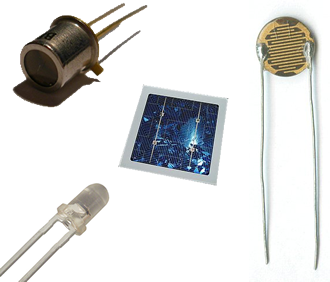
\includegraphics[width = 1\linewidth]{fig/Optica/Light_sensor.png}
            \tiny{Tomado de \cite{Fraden_2016}}
        \end{column}
    \end{columns}
\end{frame}

\begin{frame}{Fotodiodos}
    \begin{columns}[onlytextwidth]
        \begin{column}{0.55\textwidth}
            \begin{itemize}
                \item Sensores ópticos (los paneles solares funcionan de la misma forma).
                \item Cuando un haz de luz es dirigido hacia el sensor, generará una fotocorriente. La cual puede ser medida mediante un circuito de acople de corriente. 
                \item La corriente está dada por: 
                \begin{equation*}
                    i=i_{0}(e^{\frac{eV}{K_bT}-1})-i_s
                \end{equation*}
            \end{itemize}
        \end{column}
        \begin{column}{0.45\textwidth}
            \centering
            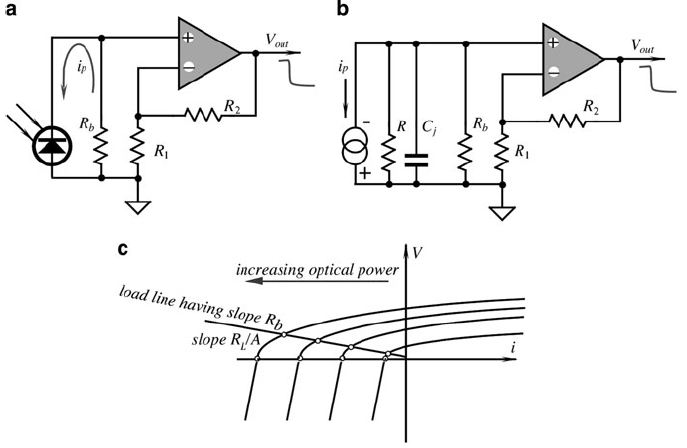
\includegraphics[width = 1\linewidth]{fig/Optica/fotodiodos.PNG}
            \tiny{Tomado de \cite{Fraden_2016}}
            \tiny{Conexión de un fotodiodo a) circuito equivalente, b)circuito de carga}
        \end{column}
    \end{columns}
\end{frame}

\begin{frame}{Fototransistor}
    \begin{columns}[onlytextwidth]
        \begin{column}{0.55\textwidth}
            \begin{itemize}
                \item De forma adicional de los fotodiodos, los fototransistores pueden aportar ganancia, lo cual se traduce en mayor sensibilidad. 
                \item Tienen mucha utilidad para detectar luz infrarroja. 
                \item Pueden ser sensores de dos o tres "patas". Por lo regular la base del transistor no está conectada, ya que la luz incidente funciona como corriente de base.
            \end{itemize}
        \end{column}
        \begin{column}{0.45\textwidth}
            \centering
            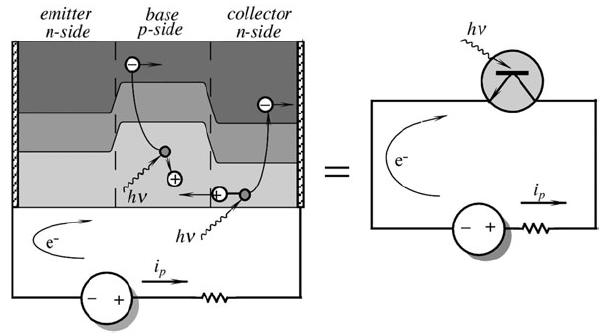
\includegraphics[width = 0.9\linewidth]{fig/Optica/fototransistor.PNG}
            \tiny{Tomado de \cite{Fraden_2016}}
            \tiny{Bandas energéticas en el transistor}
        \end{column}
    \end{columns}
\end{frame}

\begin{frame}{Fotoresistor}
    \begin{columns}[onlytextwidth]
        \begin{column}{0.55\textwidth}
            \begin{itemize}
                \item Son sensores fotoeléctricos. Pero en este caso, la resistencia varía en función de la cantidad de luz que incide sobre la superficie. 
                \item Estos sensores si necesitan una fuente externa de corriente, ya que no pueden generar electricidad como los fotodiodos o fototransistores.  
                \item Los materiales más utilizados son sulfuro de cadmio (CdS) y cadmio selenio (CdSe)
            \end{itemize}
        \end{column}
        \begin{column}{0.45\textwidth}
            \centering
            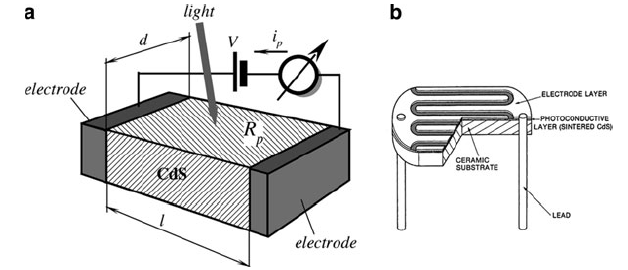
\includegraphics[width = 1\linewidth]{fig/Optica/fotoresistores.PNG}
            \tiny{Tomado de \cite{Fraden_2016}}
            \tiny{Conexión de un fotodiodo a) circuito equivalente, b)circuito de carga}
        \end{column}
    \end{columns}
\end{frame}

\begin{frame}{Comparativa entre detectores}
    \begin{table}[]
 \footnotesize
    \centering
    \begin{tabular}{m{2.6cm} m{3.8cm} m{3.8cm}}
        \toprule
        \textbf{Tipo de Sensor} & \textbf{Características} & \textbf{Ejemplos de estructuras}\\
        \midrule
        \textbf{Fotodiodos} & Basados en uniones pn & Diodos pn, fotodiodos de valancha, fotodiodos de heterounión\\
        \textbf{Fototransistores} & Transistores sensibles a la luz, amplifican la corriente eléctrica por variaciones de luz existentes & npn BJT, pnp BJT\\
        \textbf{Detectores fotoconductivos} & Varian su conductividad debido a la absorpción de luz existente & LDR (resistencia dependiente de luz), IR (detector de infrarrojo) \\

        \bottomrule
    \end{tabular}
    \tiny{\caption{Comparación entre distintos sensores ópticos} \cite{sole2005instrumentacion}}
    \label{tab:Comparacion_sensores}
\end{table}
\end{frame}


\begin{frame}{Transmisión, fuentes y detectores de luz}
    \begin{columns}[c, onlytextwidth]
        \begin{column}{0.6\textwidth}
            \begin{itemize}
                \item En la industria es muy normal la utilización de sensores tipo barrera.
                \item Consisten en un emisor y un receptor de espectro de medición visible o infrarroja.
                \item Se utilizan para medir el cambio en la cantidad de luz causado por un objeto al cruzar el eje óptico.
            \end{itemize}
        \end{column}
        \begin{column}{0.40\textwidth}
            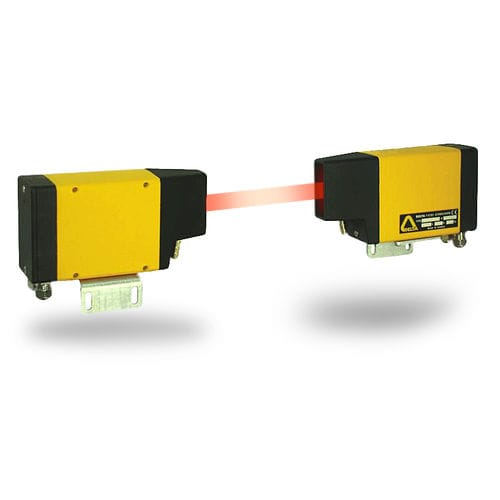
\includegraphics[width = 1\linewidth]{fig/Optica/barrera.jpg}

            \tiny{Tomado de \href{https://www.directindustry.es/prod/delta/product-68641-561968.html}{acá}}
        \end{column}
    \end{columns}
\end{frame}

\begin{frame}{Microscopio de barrido electrónico}
    \begin{columns}[c, onlytextwidth]
    \begin{column}{0.45\textwidth}
            \centering
            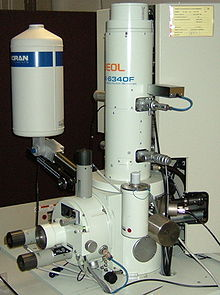
\includegraphics[width = 0.7\linewidth]{fig/Optica/microscopio.jpg}\\
            \tiny{Tomado de: \href{https://es.wikipedia.org/wiki/Microscopio_electrónico_de_barrido}{Wikicommons}}
        \end{column}
        \begin{column}{0.55\textwidth}
            \begin{itemize}
                \item Es un microscopio electrónico capaz de producir imágenes de alta resolución.
                \item Para ello, se utiliza la interacción electrón-materia.
                \item Se aplica un haz de electrones para formar una imagen.
                \item Las técnicas actuales permiten la obtención de imágenes de alta definición y en 3D.
            \end{itemize}
        \end{column}
    \end{columns}
\end{frame}

\begin{frame}{Microscopio de barrido electrónico}
    \centering
    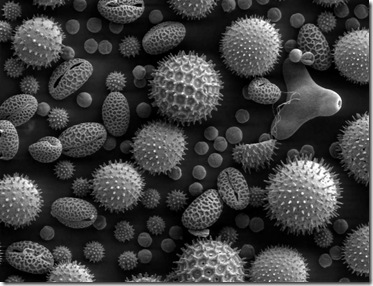
\includegraphics[width=8cm]{fig/Optica/Microscopia.jpg}
     \tiny{Tomado de: \href{https://cienciaexplicada.com/microscopio-electronico-de-barrido.html}{Acá}}
\end{frame}



\begin{frame}{Referencias}
\bibliographystyle{ieeetr}
\footnotesize
\bibliography{comunes/referencias}
\end{frame}

\end{document}